%contient des exemples d'homographies traité par nous et ripmap

\sse{Comparaison du Ripmap et de la décomposition géométrique}

Cette section décrit succintement les expériences représentées aux figures \ref{Homo1}, \ref{Homo2}, \ref{Homo3}, \ref{Homo4}, \ref{Homo5} et \ref{Homo5det}. On a choisit des homographies éloignées des cas dégénérés.

On peut remarquer que la décomposition permet pour certaines homographies de limiter l'\emph{aliasing} (Homographies 1 ,4 et 5). Dans le cas d'une déformation en diagonale elle limite le flou (Homographie 2). Il existe néanmoins des cas où les deux méthodes ont des performances comparables (Homographie 3).

Le programme a un temps d'éxecution de l'ordre d'une seconde sur une image $512\times 512$ avec un laptop à deux processeurs.

\begin{figure}
\subfigure[Décomposition géométrique]{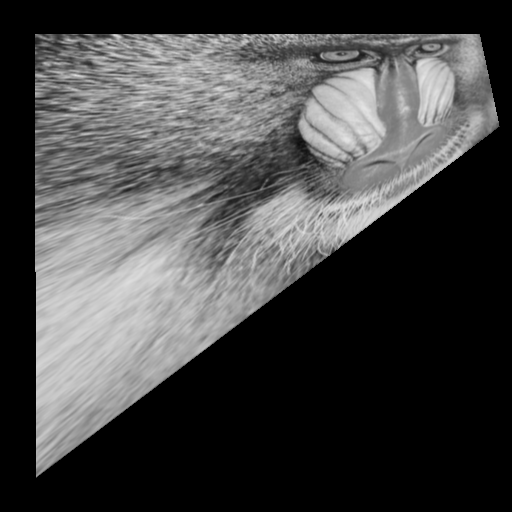
\includegraphics[scale=0.4]{img_f_1.png}}
\subfigure[Ripmap]{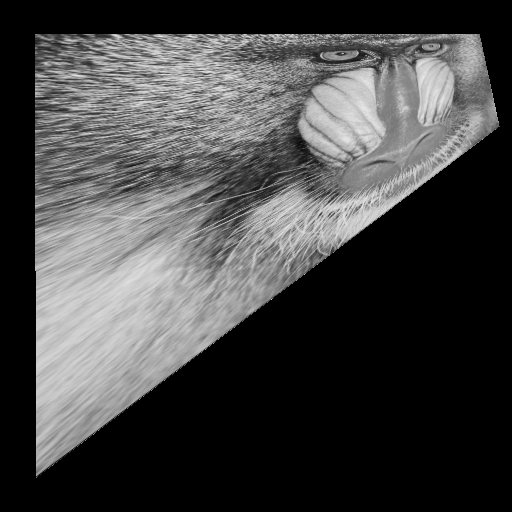
\includegraphics[scale=0.4]{img_ripmap_1.png}}
\caption{Homographie 1 : La décomposition géométrique produit moins d'\emph{aliasing}}
\label{Homo1}
\end{figure}

\begin{figure}
\subfigure[Décomposition géométrique]{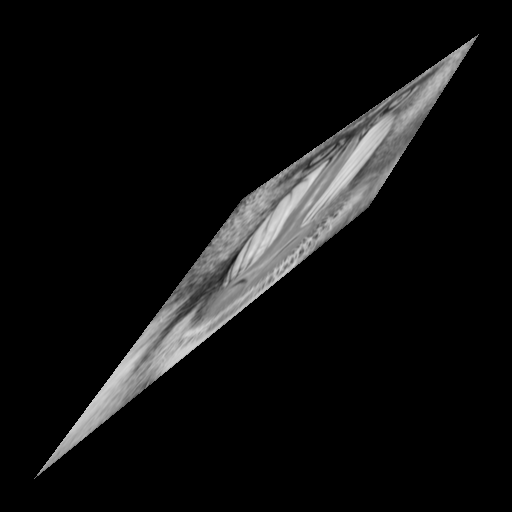
\includegraphics[scale=0.4]{img_f_2.png}}
\subfigure[Ripmap]{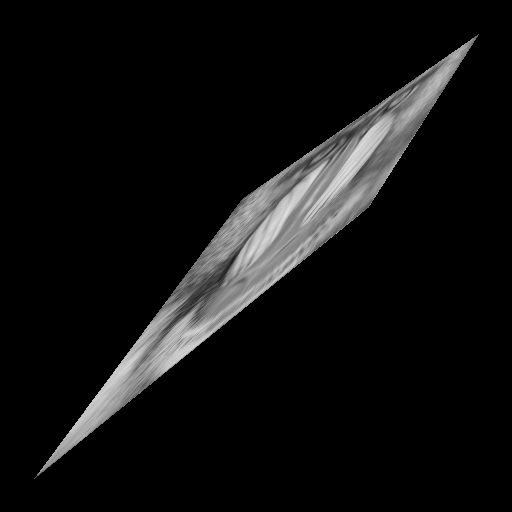
\includegraphics[scale=0.4]{img_ripmap_2.png}}
\caption{Homographie 2 : La décomposition n'entraine pas d'\emph{over-blurring} (voir section \ref{Ripmap})}
\label{Homo2}
\end{figure}

\begin{figure}
\subfigure[Décomposition géométrique]{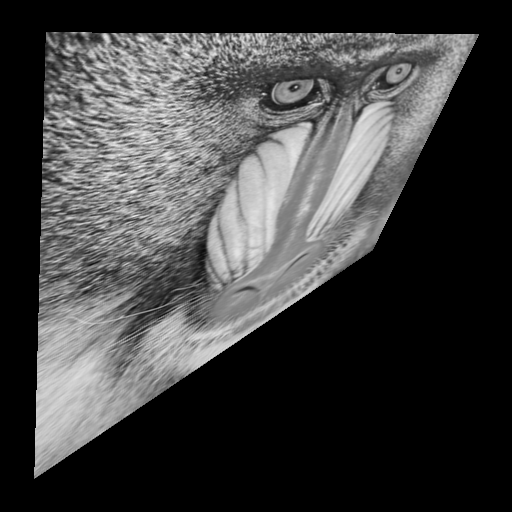
\includegraphics[scale=0.4]{img_f_3.png}}
\subfigure[Ripmap]{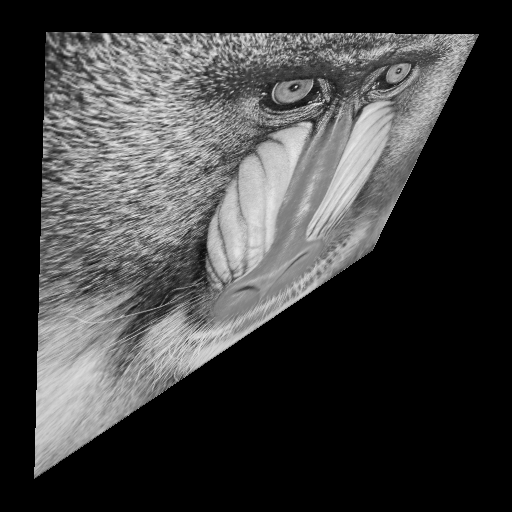
\includegraphics[scale=0.4]{img_ripmap_3.png}}
\caption{Homographie 3 : Aucune des deux méthodes n'est clairement meilleure}
\label{Homo3}
\end{figure}

\begin{figure}
\subfigure[Décomposition géométrique]{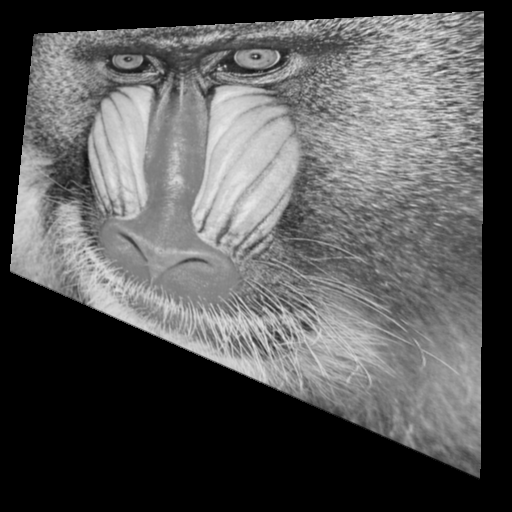
\includegraphics[scale=0.4]{img_f_4.png}}
\subfigure[Ripmap]{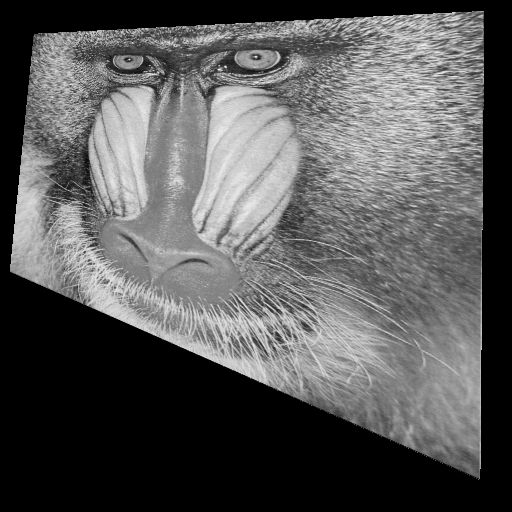
\includegraphics[scale=0.4]{img_ripmap_4.png}}
\caption{Homographie 4 : La décomposition géométrique produit moins d'\emph{aliasing}}
\label{Homo4}
\end{figure}

\begin{figure}
\subfigure[Décomposition géométrique]{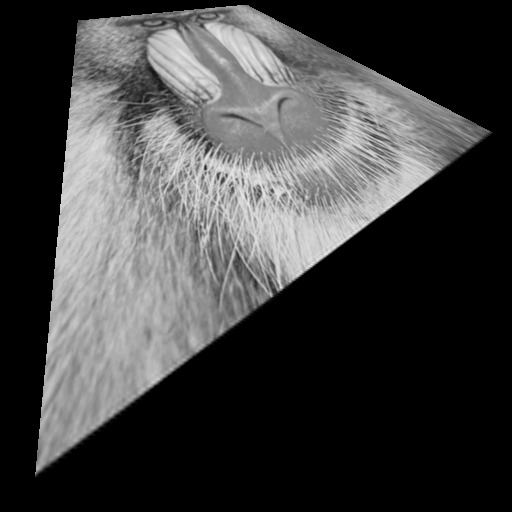
\includegraphics[scale=0.4]{img_geo_5.png}}
\subfigure[Ripmap]{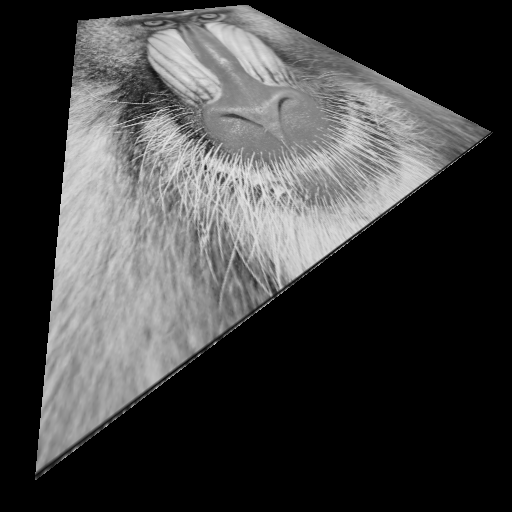
\includegraphics[scale=0.4]{img_ripmap_5.png}}
\subfigure[Méthode naive]{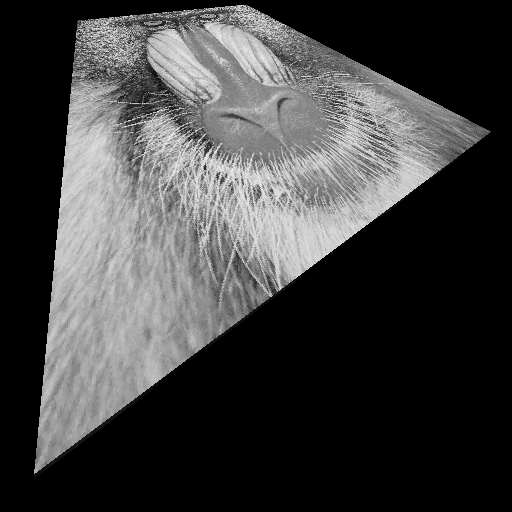
\includegraphics[scale=0.4]{img_naive_5.png}}
\subfigure[Mipmap]{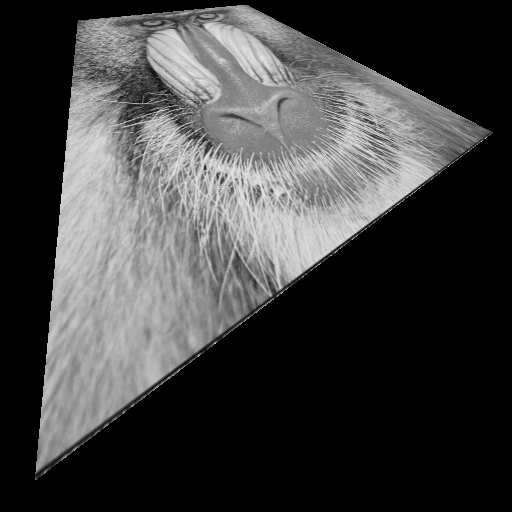
\includegraphics[scale=0.4]{img_mipmap_5.png}}
\caption{Homographie 5 : La décomposition produit moins d'aliasing, un détail est présenté dans la figure \ref{Homo5det}}
\label{Homo5}
\end{figure}

\begin{figure}[t]
\centering
\subfigure[Méthode naive]{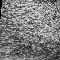
\includegraphics[scale=1.25]{img_det_naive.png}}\hfill
\subfigure[Mipmap]{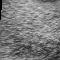
\includegraphics[scale=1.25]{img_det_mipmap.png}}\hfill
\subfigure[Ripmap]{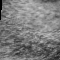
\includegraphics[scale=1.25]{img_det_ripmap.png}}\hfill
\subfigure[Décomposition géométrique]{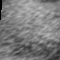
\includegraphics[scale=1.25]{img_det_geo.png}}
\caption{Détail de l'homographie 5 qui a été présentée dans la figure \ref{Homo5} }
\label{Homo5det}
\end{figure}
